\begin{evenBlock}{2 vs. 1 Offense}


\begin{minipage}[t]{\linewidth}
    \centering
    
    \begin{minipage}{.3\linewidth} % Left column and width
        %\begin{figure}
            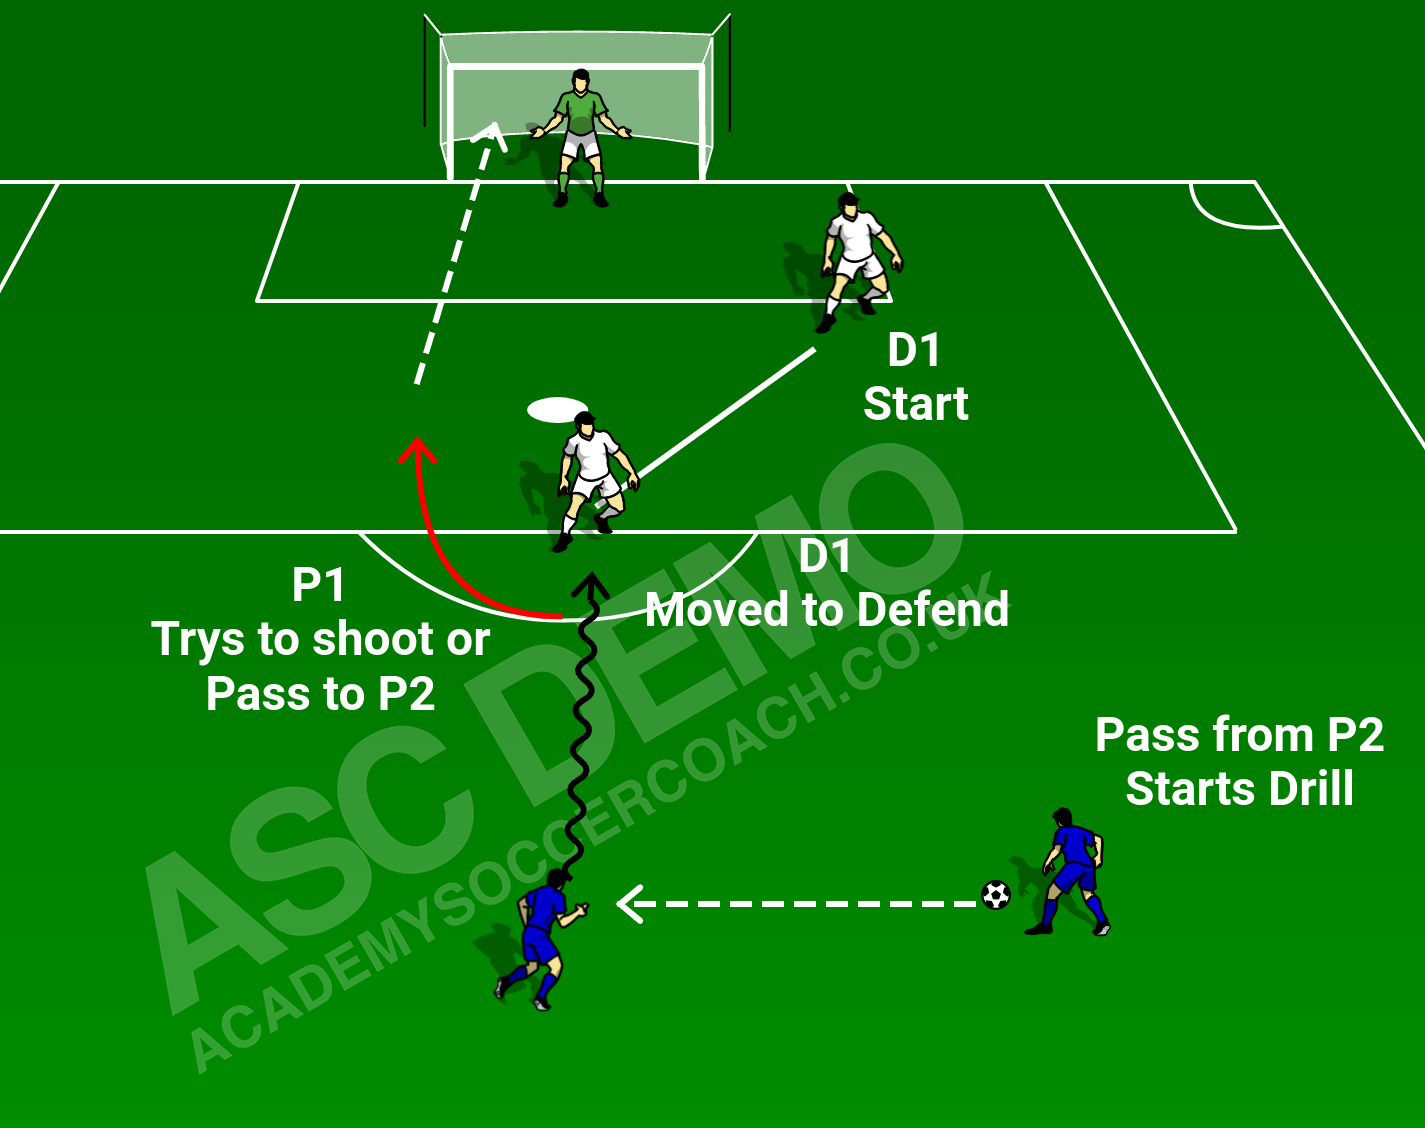
\includegraphics[width=\textwidth]{../img/Trimmed/2v1_Option}

            \vspace{3pt}
            
            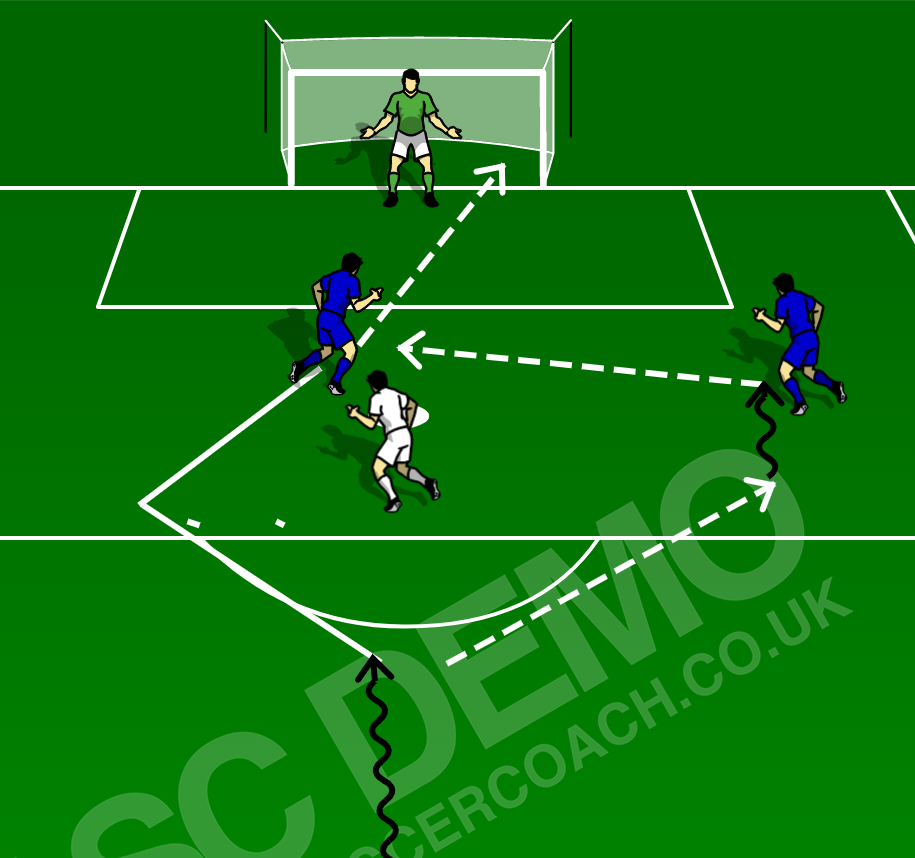
\includegraphics[width=\textwidth]{../img/Trimmed/2v1_Option_Pass}
        %    \caption{Drill: 4 Person Passing}
        %\end{figure}
    \end{minipage}
    \hspace{0.05\linewidth}
    \begin{minipage}{.6\linewidth} % Left column and width
        \textbf{Drill Description:}
        This drill is designed train the forward to make a quick decision on how to beat a defender.  He has two options, dribble around the defender or pass to his wing and make a move around the defender. 
        \begin{enumerate}
        \setlength{\itemsep}{0pt}
        \setlength{\parskip}{0pt}
        \setlength{\parsep}{0pt}
        \item The wing (P2) starts the play by passing to the forward.  The defender (D1) starts at the corner of the 6 yard box.
        \item The forward drives to goal as a defender come charging to defend.
        \item The forward has two choices, pass or make a move/touch around the defender.
        \item The goal is to get a shot on goal.
        \item If he passes the ball, the wing should cross the ball quickly as the striker is passing the defender.
        \end{enumerate}

        \vspace{3pt}
        
        Rotate rolls each shot: P2 to P1, P1 to D1, D1 to P2.

        \vspace{10pt}
        
        \textbf{Coaching Points:}
        \begin{itemize}
        \setlength{\itemsep}{0pt}
        \setlength{\parskip}{0pt}
        \setlength{\parsep}{0pt}
        \item The forward needs to decide quickly which option he plans to take.
        \item The wing needs to be ready at all times and should stay `on-side'.
        \item The forward should try and take advantage of any weakness of the defense, or try and create weakness by using a scissor move or a fake.
        \item Explain on-sides and off-sides.
        \end{itemize}

    \end{minipage}
\end{minipage}

\end{evenBlock}